\begin{minipage}{0.15\linewidth}
    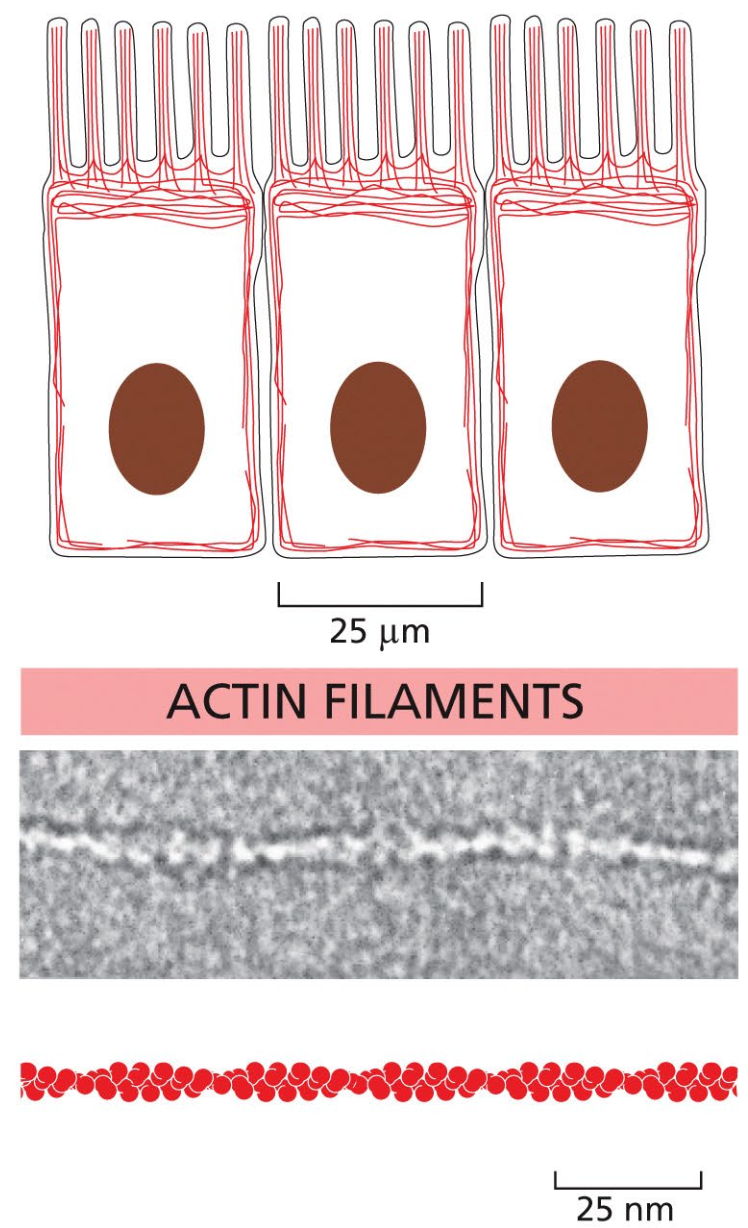
\includegraphics[width=15mm]{src/Images/actin.png}
\end{minipage}
\begin{minipage}{0.85\linewidth}
\begin{itemize}
    \item Provide \textbf{support}, change the \textbf{cell shape} (division) and drive \textbf{movement}
    \item Assemble from \textbf{globular proteins} (“G-Actin”) like microtubules and form \textbf{hierarchical structures} bycrosslinking
    \item \textbf{Polar} with \textbf{no preferred direction}
    \item Can form \textbf{protrusions} → \textbf{exploring} and \textbf{sensing environment}
    \item \textbf{“Myosin motors”} → participate in cargo transport and muscle contraction
\end{itemize}
\end{minipage}\\

\textbf{Muscle contraction:} \hfill $\delta W = F \cdot d x$ \\
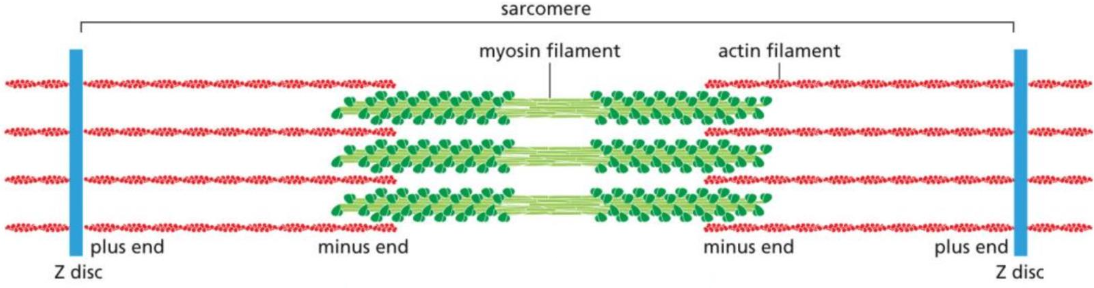
\includegraphics[width=60mm]{src/Images/muscle_contraction.png}\\
In a \textbf{sarcomere}, \textbf{myosin II} binds to actin and \textbf{proceeds towards the + side}.\\
This sliding of myosin on actin filaments \textbf{shortens the strands} and leads to muscle contraction
